% 非互換なパッケージに自動でパッチを当てる
% https://qiita.com/wtsnjp/items/76557b1598445a1fc9da
\RequirePackage{plautopatch}
% pdfpagesの依存パッケージのエラー回避
% https://okumuralab.org/tex/mod/forum/discuss.php?d=2956
% https://github.com/aminophen/gentombow/issues/9
\plautopatchdisable{eso-pic}
% documentclassでdvipdfmx指定をするので個別パッケージでのドライバ指定は不要
% https://qiita.com/Aruneko/items/13e015bce0112143f277
\documentclass[autodetect-engine, dvi=dvipdfmx, 10pt, a4paper, ja=standard]{bxjsarticle}

% 印刷時の用紙サイズ設定
\usepackage{bxpapersize}% これでOK!

% pdf-version
\usepackage[1.4]{bxpdfver}

% 日本語環境での字体修正
\usepackage{otf}
% フォントエンコーディングの名前をオプションで指定する
\usepackage[T1]{fontenc}
\usepackage{lmodern}% Latin Modern フォントを使う

% graphicx
\usepackage{graphicx}
\usepackage{grffile}% include graphicsの画像ファイル名の制限を撤廃

% \begin{comment} ... \end{comment} で複数行コメントアウト
\usepackage{comment}

% 数学系 インライン数式を \[ \] と書く癖をつける
\usepackage{amsmath,amssymb,amsthm}
\usepackage{amsfonts}
\usepackage{mathtools}
\usepackage{bm} % bold math

% 化学
\usepackage[version=4]{mhchem}

% SI単位系
\usepackage{siunitx}

% 表関連
\usepackage{multirow} % 表のセルの結合
\usepackage{booktabs} % 表の線がすごくなる. Table Generatorを使うときはbooktabsモードにする
\usepackage{caption} % キャプションをいじる
\usepackage{float} % 図表を絶対にそこに置く確固たる意思

% その他便利な子
\usepackage{pdfpages} % pdfを挿入
\usepackage[hyphens]{url} % urlをきれいに表示する
\usepackage{ulem} % 下線を強化
\usepackage[at]{easylist} % @をつかって箇条書き
% \usepackage{minted}
% \usepackage{termsim} % ターミナルを再現...誰得?

% ハイパーリンクを生成
% sectionなどで数式を使う場合は \texorpdfstring{texstring}{pdfstring}をする
\usepackage{hyperref}
\usepackage{pxjahyper}
\usepackage{footnotebackref} % 脚注から本文へ飛べる


% ここからはソースコードを表示する設定
\usepackage{listings, plistings, color}
\renewcommand{\lstlistingname}{Code}
\definecolor{OliveGreen}{rgb}{0.0,0.6,0.0}
\definecolor{Orenge}{rgb}{0.89,0.55,0}
\definecolor{SkyBlue}{rgb}{0.28, 0.28, 0.95}
\lstset{
    language={Ruby}, % 言語の指定
    basicstyle={\ttfamily},
    identifierstyle={\small},
    commentstyle={\smallitshape},
    keywordstyle={\small\bfseries},
    ndkeywordstyle={\small},
    stringstyle={\small\ttfamily},
    frame={tb},
    breaklines=true,
    columns=[l]{fullflexible},
    numbers=left,
    xrightmargin=0zw,
    xleftmargin=3zw,
    numberstyle={\scriptsize},
    stepnumber=1,
    numbersep=1zw,
    lineskip=-0.5ex,
    stepnumber=1,       % 行数の増間
    numbersep=1zw,      % 行数の余白
    xrightmargin=0zw,   % 左の余白
    xleftmargin=2zw,    % 右の余白
    framexleftmargin=18pt,  % フレームからの左の余白
    keepspaces=true,    % スペースを省略せず保持
    lineskip=-0.2ex,    % 枠線の途切れ防止
    tabsize = 4,        % タブ数
    showstringspaces=false,  %文字列中の半角スペースを表示させない
    keywordstyle={\color{SkyBlue}},     %キーワード(int, ifなど)の書体指定
    commentstyle={\color{OliveGreen}},  %注釈の書体
    stringstyle=\color{Orenge}          %文字列
}

% \refだけで「図」や「式」を自動挿入
% https://zenn.dev/arks/articles/3697b25d03f8a8
% subfigureが文書にあると小節を参照する際に使う\subrefがおかしくなるので注意
%% increase link area for cross-references and autoname them, [130514]
\AtBeginDocument{\renewcommand{\ref}[1]{\mbox{\autoref{#1}}}}

\def\equationautorefname~#1\null{式(#1)\null}
\def\figureautorefname~#1\null{図#1\null}
\def\subfigureautorefname#1\null{図#1\null}
\def\tableautorefname~#1{表#1}
\def\lstlistingautorefname~#1{コード#1}

\def\partautorefname#1\null{第#1部\null}
\def\chapterautorefname#1\null{第#1章\null}
\def\sectionautorefname#1\null{#1節}
\def\subsectionautorefname~#1\null{#1節}
\def\subsubsectionautorefname#1\null{#1節}
\def\paragraphautorefname#1\null{#1段落}
\def\subparagraphautorefname#1\null{#1段落}

\def\Itemautorefname#1\null{項目#1\null}
\def\Hfootnoteautorefname#1\null{脚注#1\null}
\def\theoremautorefname#1\null{定理#1\null}
\def\FancyVerbLineautorefname#1\null{#1行\null}
% \def\pageautorefname#1\null{ページ#1\null}
\def\appendixautorefname#1\null{付録#1\null}


\title{MICS実験第一 J2課題レポート}
\author{学籍番号 2210342, 鈴木謙太郎}
\date{\today}
\begin{document}
\maketitle


\section{問題1}
\label{sec:ex-1}

\subsection{モジュールeqの動作検証}

実験資料で示された\ref{code:mod-eq}のようなモジュールeqを,同じく示されたeqSimを用いてシミュレーションした.
このモジュールeqは,入力$a,b$に対して$(a \land b) \lor (\bar{a} \land \bar{b})$を出力するもので,$a = b$のときだけ$s = 1$となる.


\begin{lstlisting}[language={Verilog}, caption={モジュールeqのVerilogコード}, label={code:mod-eq}]
module eq (
    s,a,b
);
    input a, b;
    output s;
    wire na, nb, s1, s2;
    assign na = ~a, nb = ~b;
    assign s1 = a & b, s2 = na & nb;
    assign s = s1 | s2;
endmodule
\end{lstlisting}

このモジュールeqをシミュレーションするモジュールeqSimを\ref{code:mod-eqsim}のように作成した.
このモジュールは,上のモジュールeqに対して予想される4通りの入力をすべて与えて,それぞれの出力を確認するものである.


\begin{lstlisting}[language={Verilog}, caption={モジュールeqSimのVerilogコード}, label={code:mod-eqsim}]
module eqSim; /* 一致検出回路の */
  wire s; /* シミュレーション */
  reg x, y;
  eq g1(s, x, y);
  initial
    begin
    $dumpfile("eq.vcd");
    $dumpvars(0, eqSim);
    $monitor(" %b %b  %b  %b %b", x, y,  g1.s1, g1.s2,s, $stime);
    $display(" x y s1 s2 s       time");
    x=0; y=0;
    #50 y=1;
    #50 x=1; y=0;
    #50 y=1;
    #50 $finish;
    end
endmodule
\end{lstlisting}

その結果は下のようになった.

\begin{verbatim}
x y s time
0 0 1         0
0 1 0        50
1 0 0       100
1 1 1       150
eqSim.v:15: $finish called at 200 (1s)
\end{verbatim}


また,その波形をgtkwaveで表示した結果は\ref{fig:ex1}のようになった.

\begin{figure}[H]
	\centering
	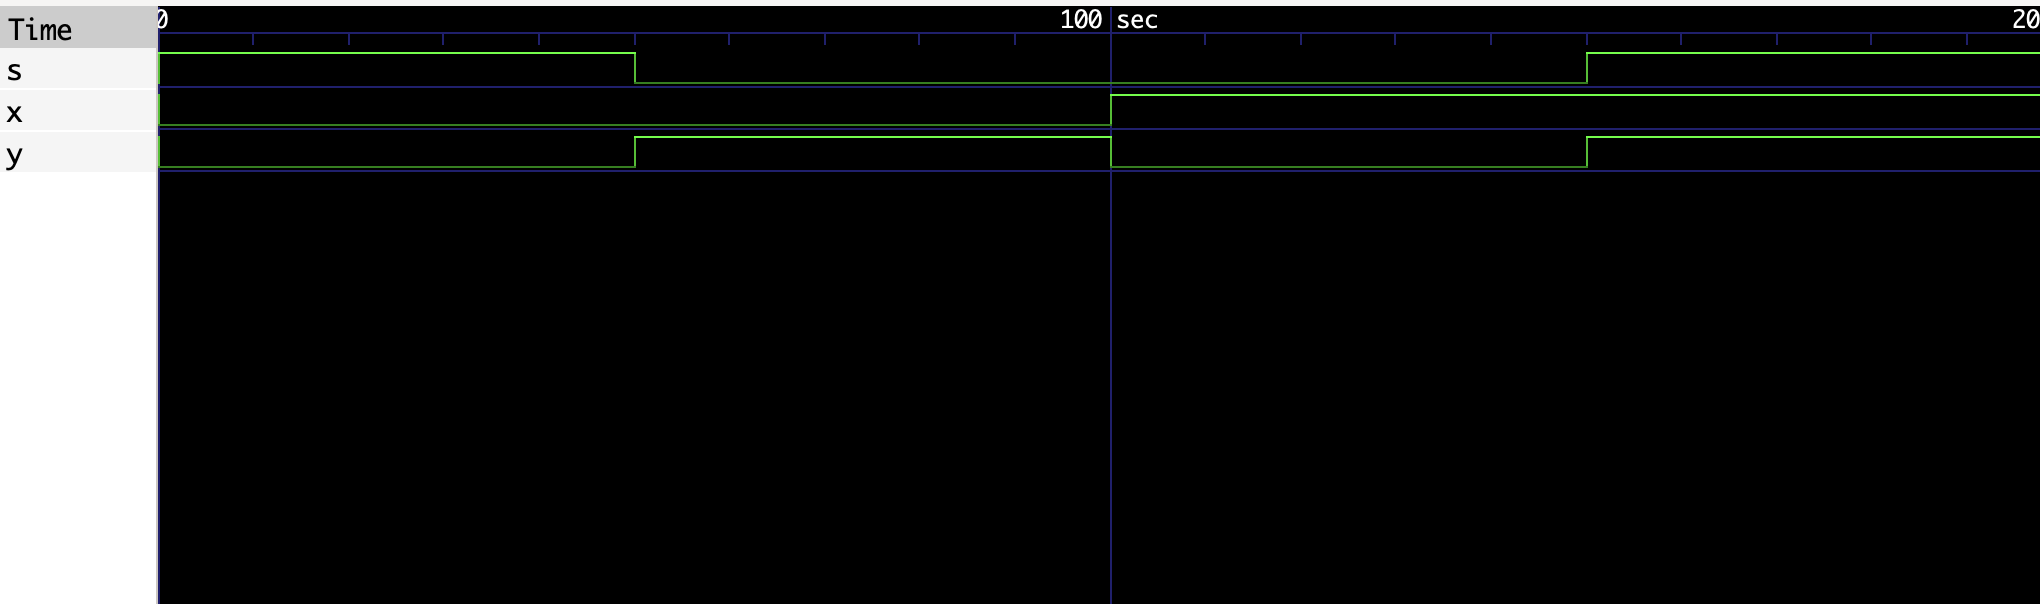
\includegraphics[width=\textwidth]{ex1.png}
	\caption{eqSimの波形}
	\label{fig:ex1}
\end{figure}

このシミュレーションはすべての入力例をカバーしており,$x=y$のときのみ$s=1$となることが確認できている.

\subsection{モジュールeqSimの改良}

モジュールeqSimを\ref{code:mod-eqsim-refined}のように改良し,eq内部の$s1, s2$を表示するようにした.

\begin{lstlisting}[language={Verilog}, caption={改良後のモジュールeqSimのVerilogコード}, label={code:mod-eqsim-refined}]
module eqSim; /* 一致検出回路の */
  wire s; /* シミュレーション */
  reg x, y;
  eq g1(s, x, y);
  initial
    begin
    $dumpfile("eq.vcd");
    $dumpvars(0, eqSim);
    $monitor(" %b %b  %b  %b %b", x, y,  g1.s1, g1.s2,s, $stime);
    $display(" x y s1 s2 s       time");
    x=0; y=0;
    #50 y=1;
    #50 x=1; y=0;
    #50 y=1;
    #50 $finish;
    end
endmodule
\end{lstlisting}

このときの出力は下のようになった.

\begin{verbatim}
x y s1 s2 s       time
0 0  0  1 1         0
0 1  0  0 0        50
1 0  0  0 0       100
1 1  1  0 1       150
eqSim.v:15: $finish called at 200 (1s)
\end{verbatim}

これにより,内部的にもs1とs2が正しく計算され,$s = s1 \lor s2$により正しい$s$が出力されていることが確認できた.

\section{問題2}
\label{sec:ex-2}

入力信号 $a, b, c, d$ を受け取り,$(a = b) \land (c = d)$のとき出力信号$s$を1に,それ以外のとき$s$を0にするモジュールdoubleEqを作成する.

このモジュールの簡易的な回路図は\ref{fig:doubleEq}のようになっている.eqと表記した部分は\ref{sec:ex-1}で扱ったモジュールeqを用いる.

\begin{figure}[H]
	\centering
	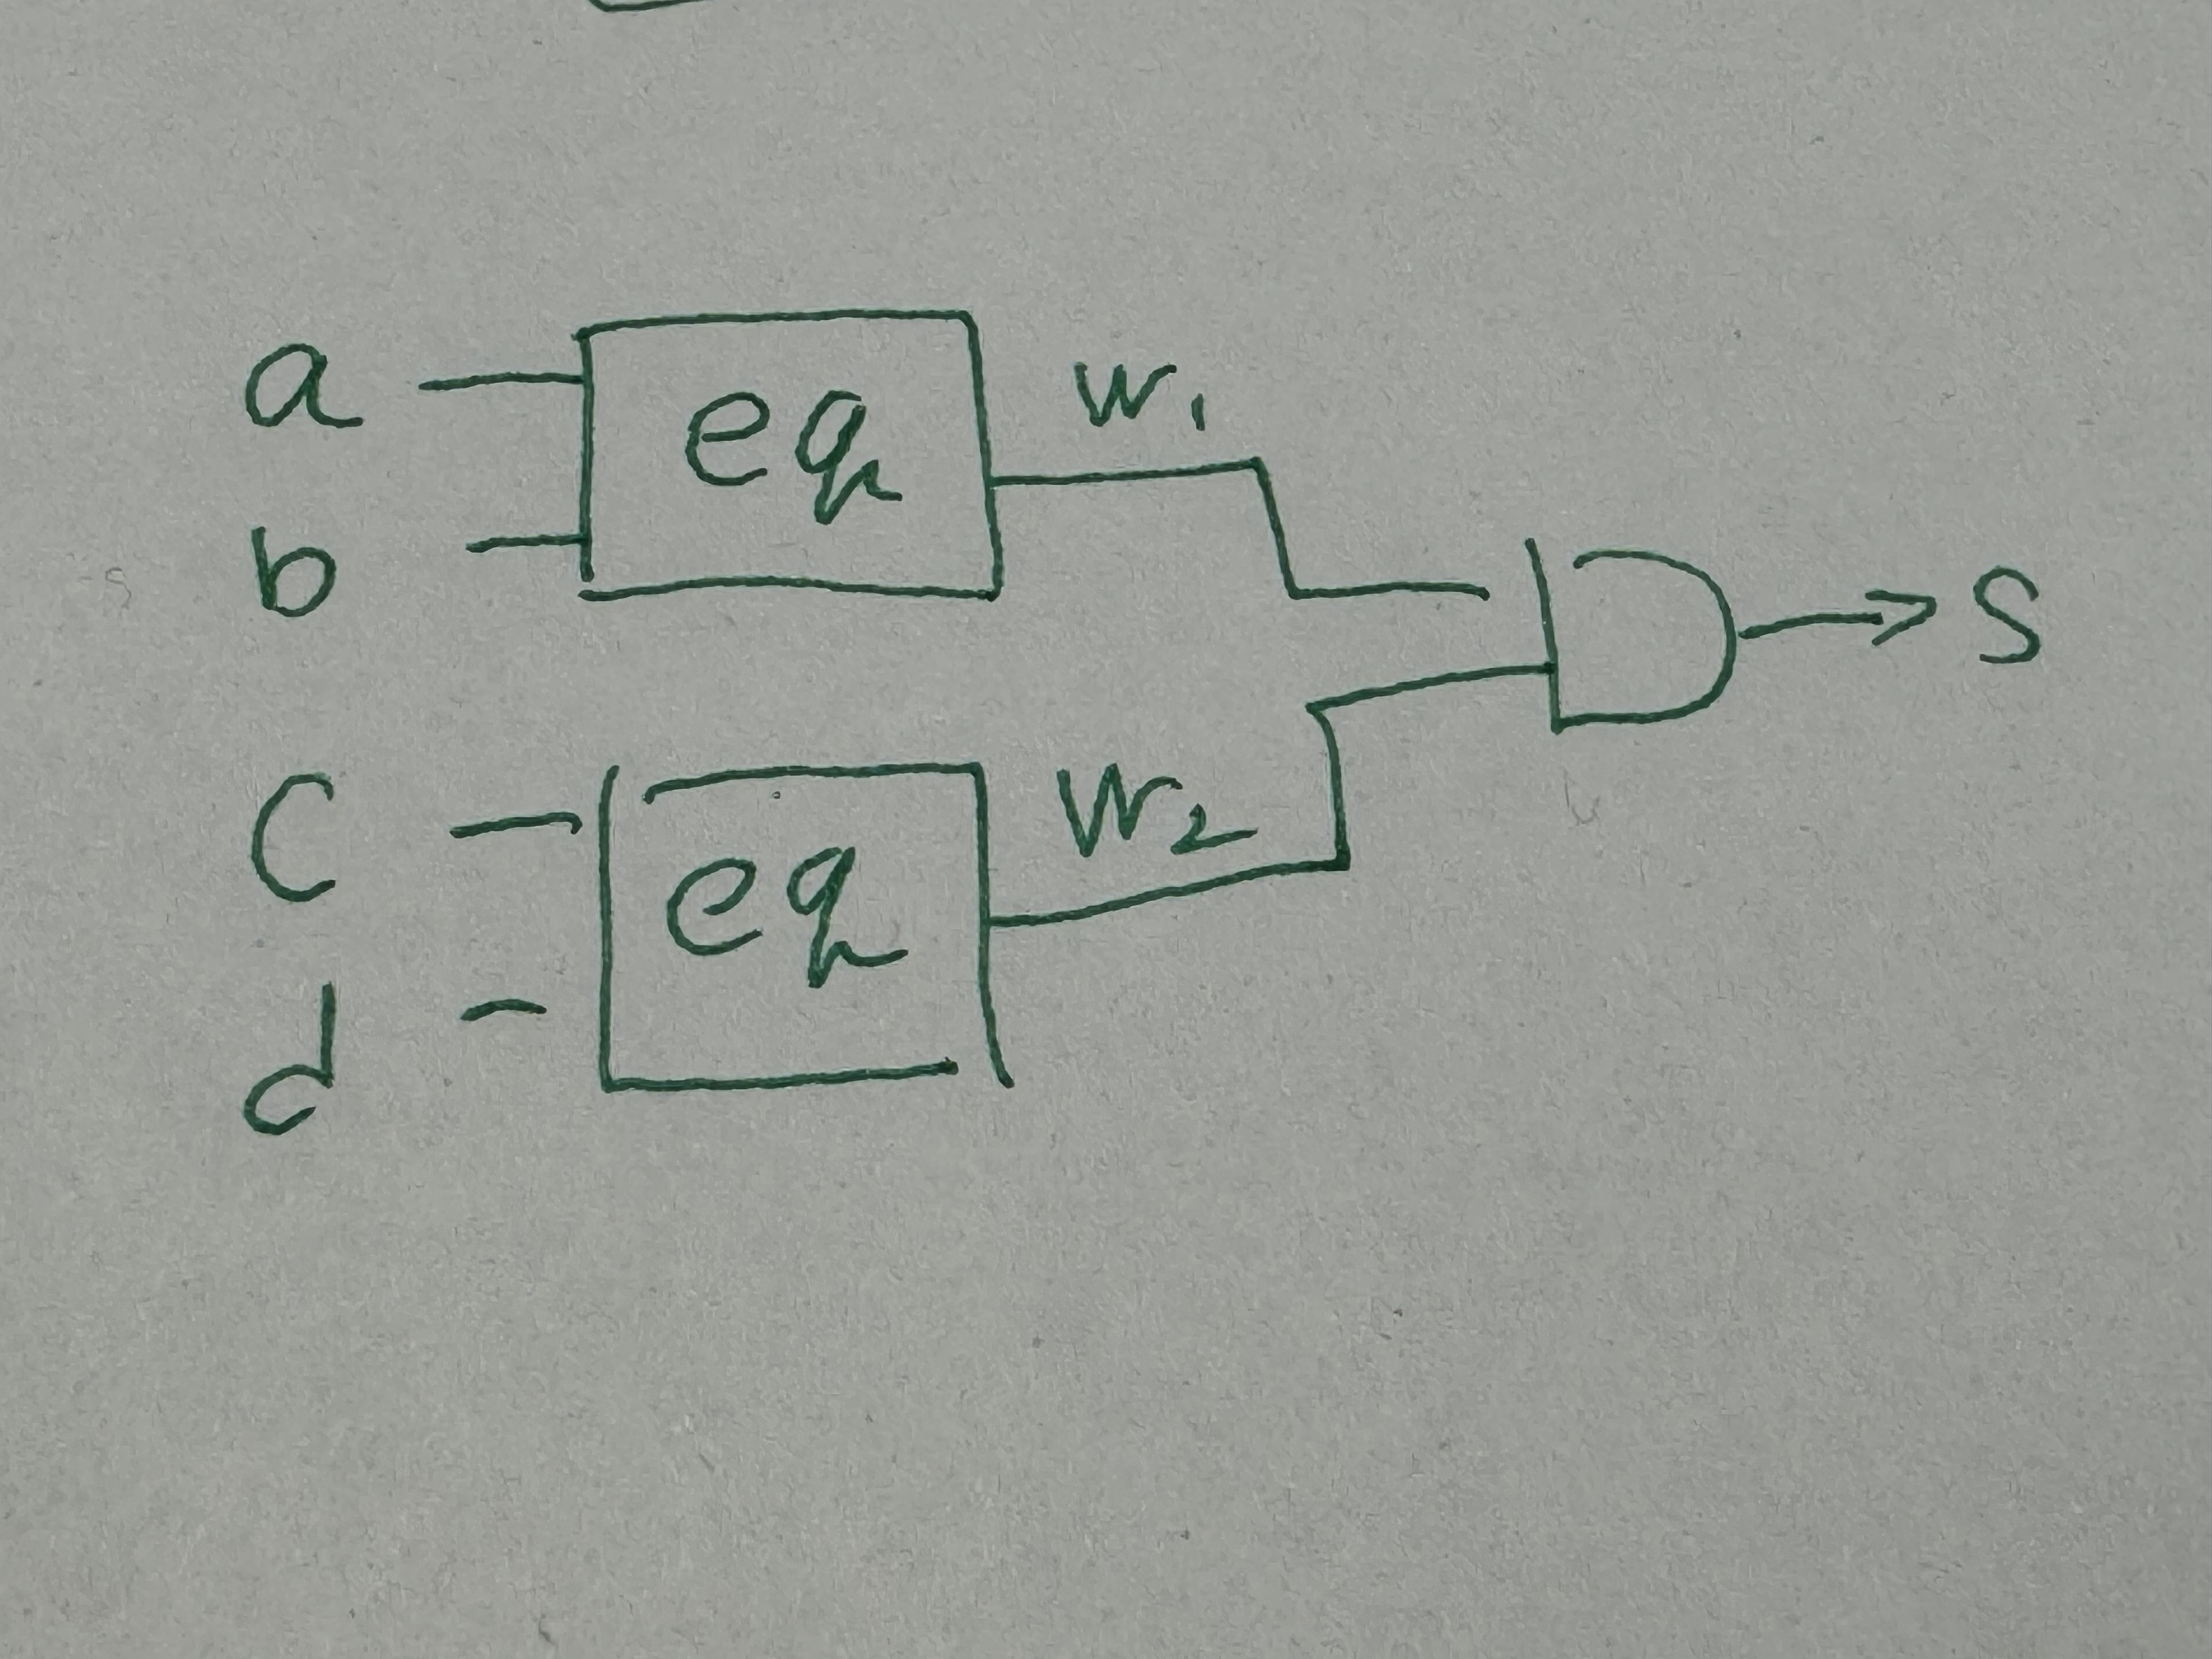
\includegraphics[width=0.8\textwidth]{ex2_kairo.jpeg}
	\caption{モジュールdoubleEqの回路図}
	\label{fig:doubleEq}
\end{figure}

これをもとに,\ref{code:mod-doubleeq}のようにモジュールdoubleEqを作成した.

\begin{lstlisting}[language={Verilog}, caption={モジュールdoubleEqのVerilogコード}, label={code:mod-doubleeq}]
module doubleEq(
    s,a,b,c,d
);
  input a, b, c, d;
  output s;
  wire w1, w2;
  eq m1(w1, a, b);
  eq m2(w2, c, d);
  assign s = w1 & w2;
endmodule
\end{lstlisting}

\section{問題3}
\label{sec:ex-3}

\ref{sec:ex-2}で作成したモジュールdoubleEqをシミュレーションするモジュールdoubleEqSimを\ref{code:mod-doubleeqsim}のように作成した.
今回は入力ケースがたかだか16通りほどだったので,想定されるすべての入力についてテストを行った.

\begin{lstlisting}[language={Verilog}, caption={モジュールdoubleEqSimのVerilogコード}, label={code:mod-doubleeqsim}]
module doubleEqSim; /* 一致検出回路の */
  wire s; /* シミュレーション */
  reg a, b, c, d;
  doubleEq g1(s, a, b, c, d);
  initial
    begin
    $dumpfile("doubleEq.vcd");
    $dumpvars(0, doubleEqSim);
    $monitor(" %b %b %b %b  %b  %b  %b", a, b, c, d, s, g1.w1, g1.w2, $stime);
    $display(" a b c d w1 w2  s      time");
    /* test all case */
    a=0; b=0; c=0; d=0;
    #50 a=0; b=0; c=0; d=1;
    #50 a=0; b=0; c=1; d=0;
    #50 a=0; b=0; c=1; d=1;
    #50 a=0; b=1; c=0; d=0;
    #50 a=0; b=1; c=0; d=1;
    #50 a=0; b=1; c=1; d=0;
    #50 a=0; b=1; c=1; d=1;
    #50 a=1; b=0; c=0; d=0;
    #50 a=1; b=0; c=0; d=1;
    #50 a=1; b=0; c=1; d=0;
    #50 a=1; b=0; c=1; d=1;
    #50 a=1; b=1; c=0; d=0;
    #50 a=1; b=1; c=0; d=1;
    #50 a=1; b=1; c=1; d=0;
    #50 a=1; b=1; c=1; d=1;
    end
endmodule
\end{lstlisting}

このテストを実行し,gtkwaveで波形を表示した結果は\ref{fig:ex3}のようになった.

\begin{figure}[H]
	\centering
	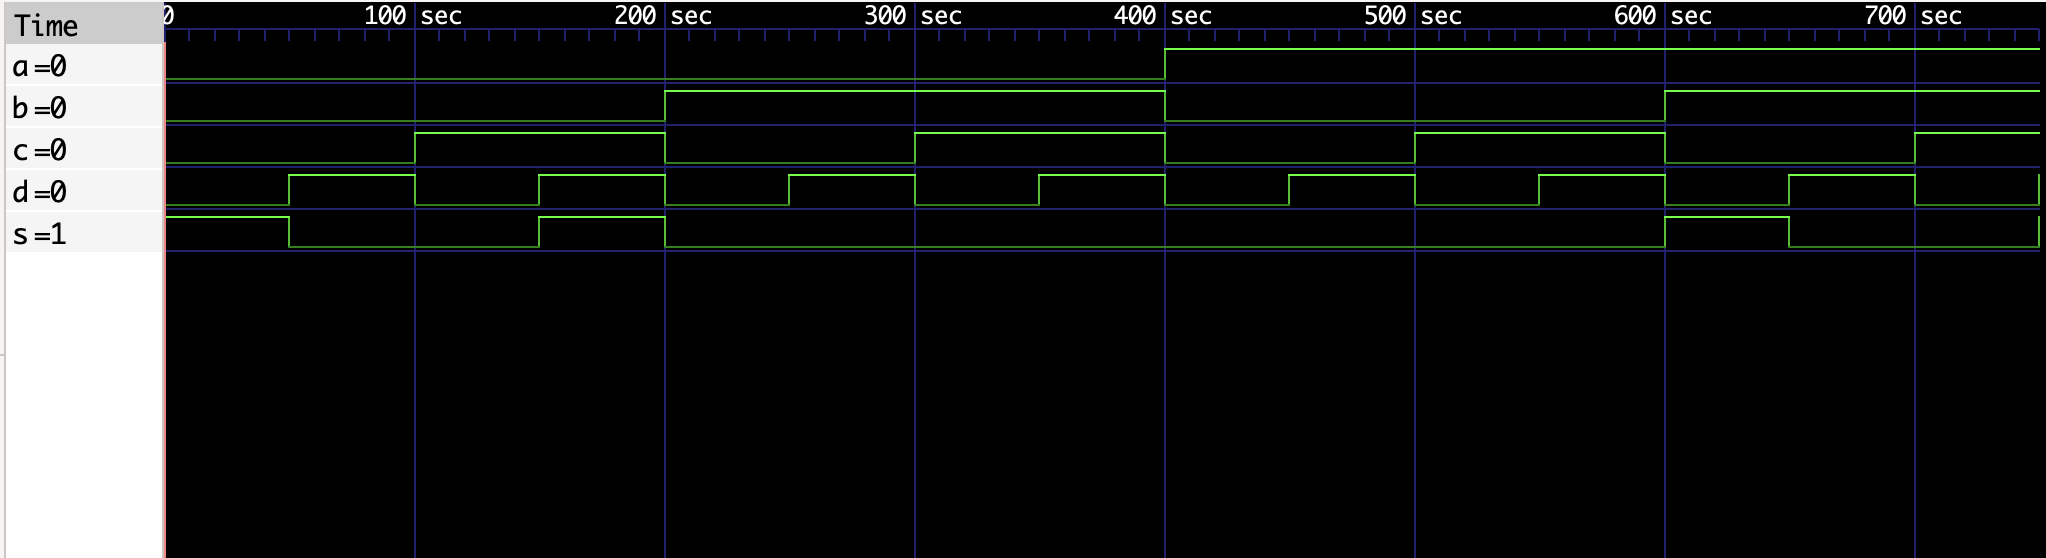
\includegraphics[width=\textwidth]{ex3.png}
	\caption{doubleEqSimの波形}
	\label{fig:ex3}
\end{figure}

この波形から,$a=b$かつ$c=d$のときだけ$s=1$となることが確認できた.

\section{問題4}

実験資料で示された状態遷移表m2に従って,\ref{fig:ex4}のような状態遷移図と真理値表を作成した.

\begin{figure}[H]
	\centering
	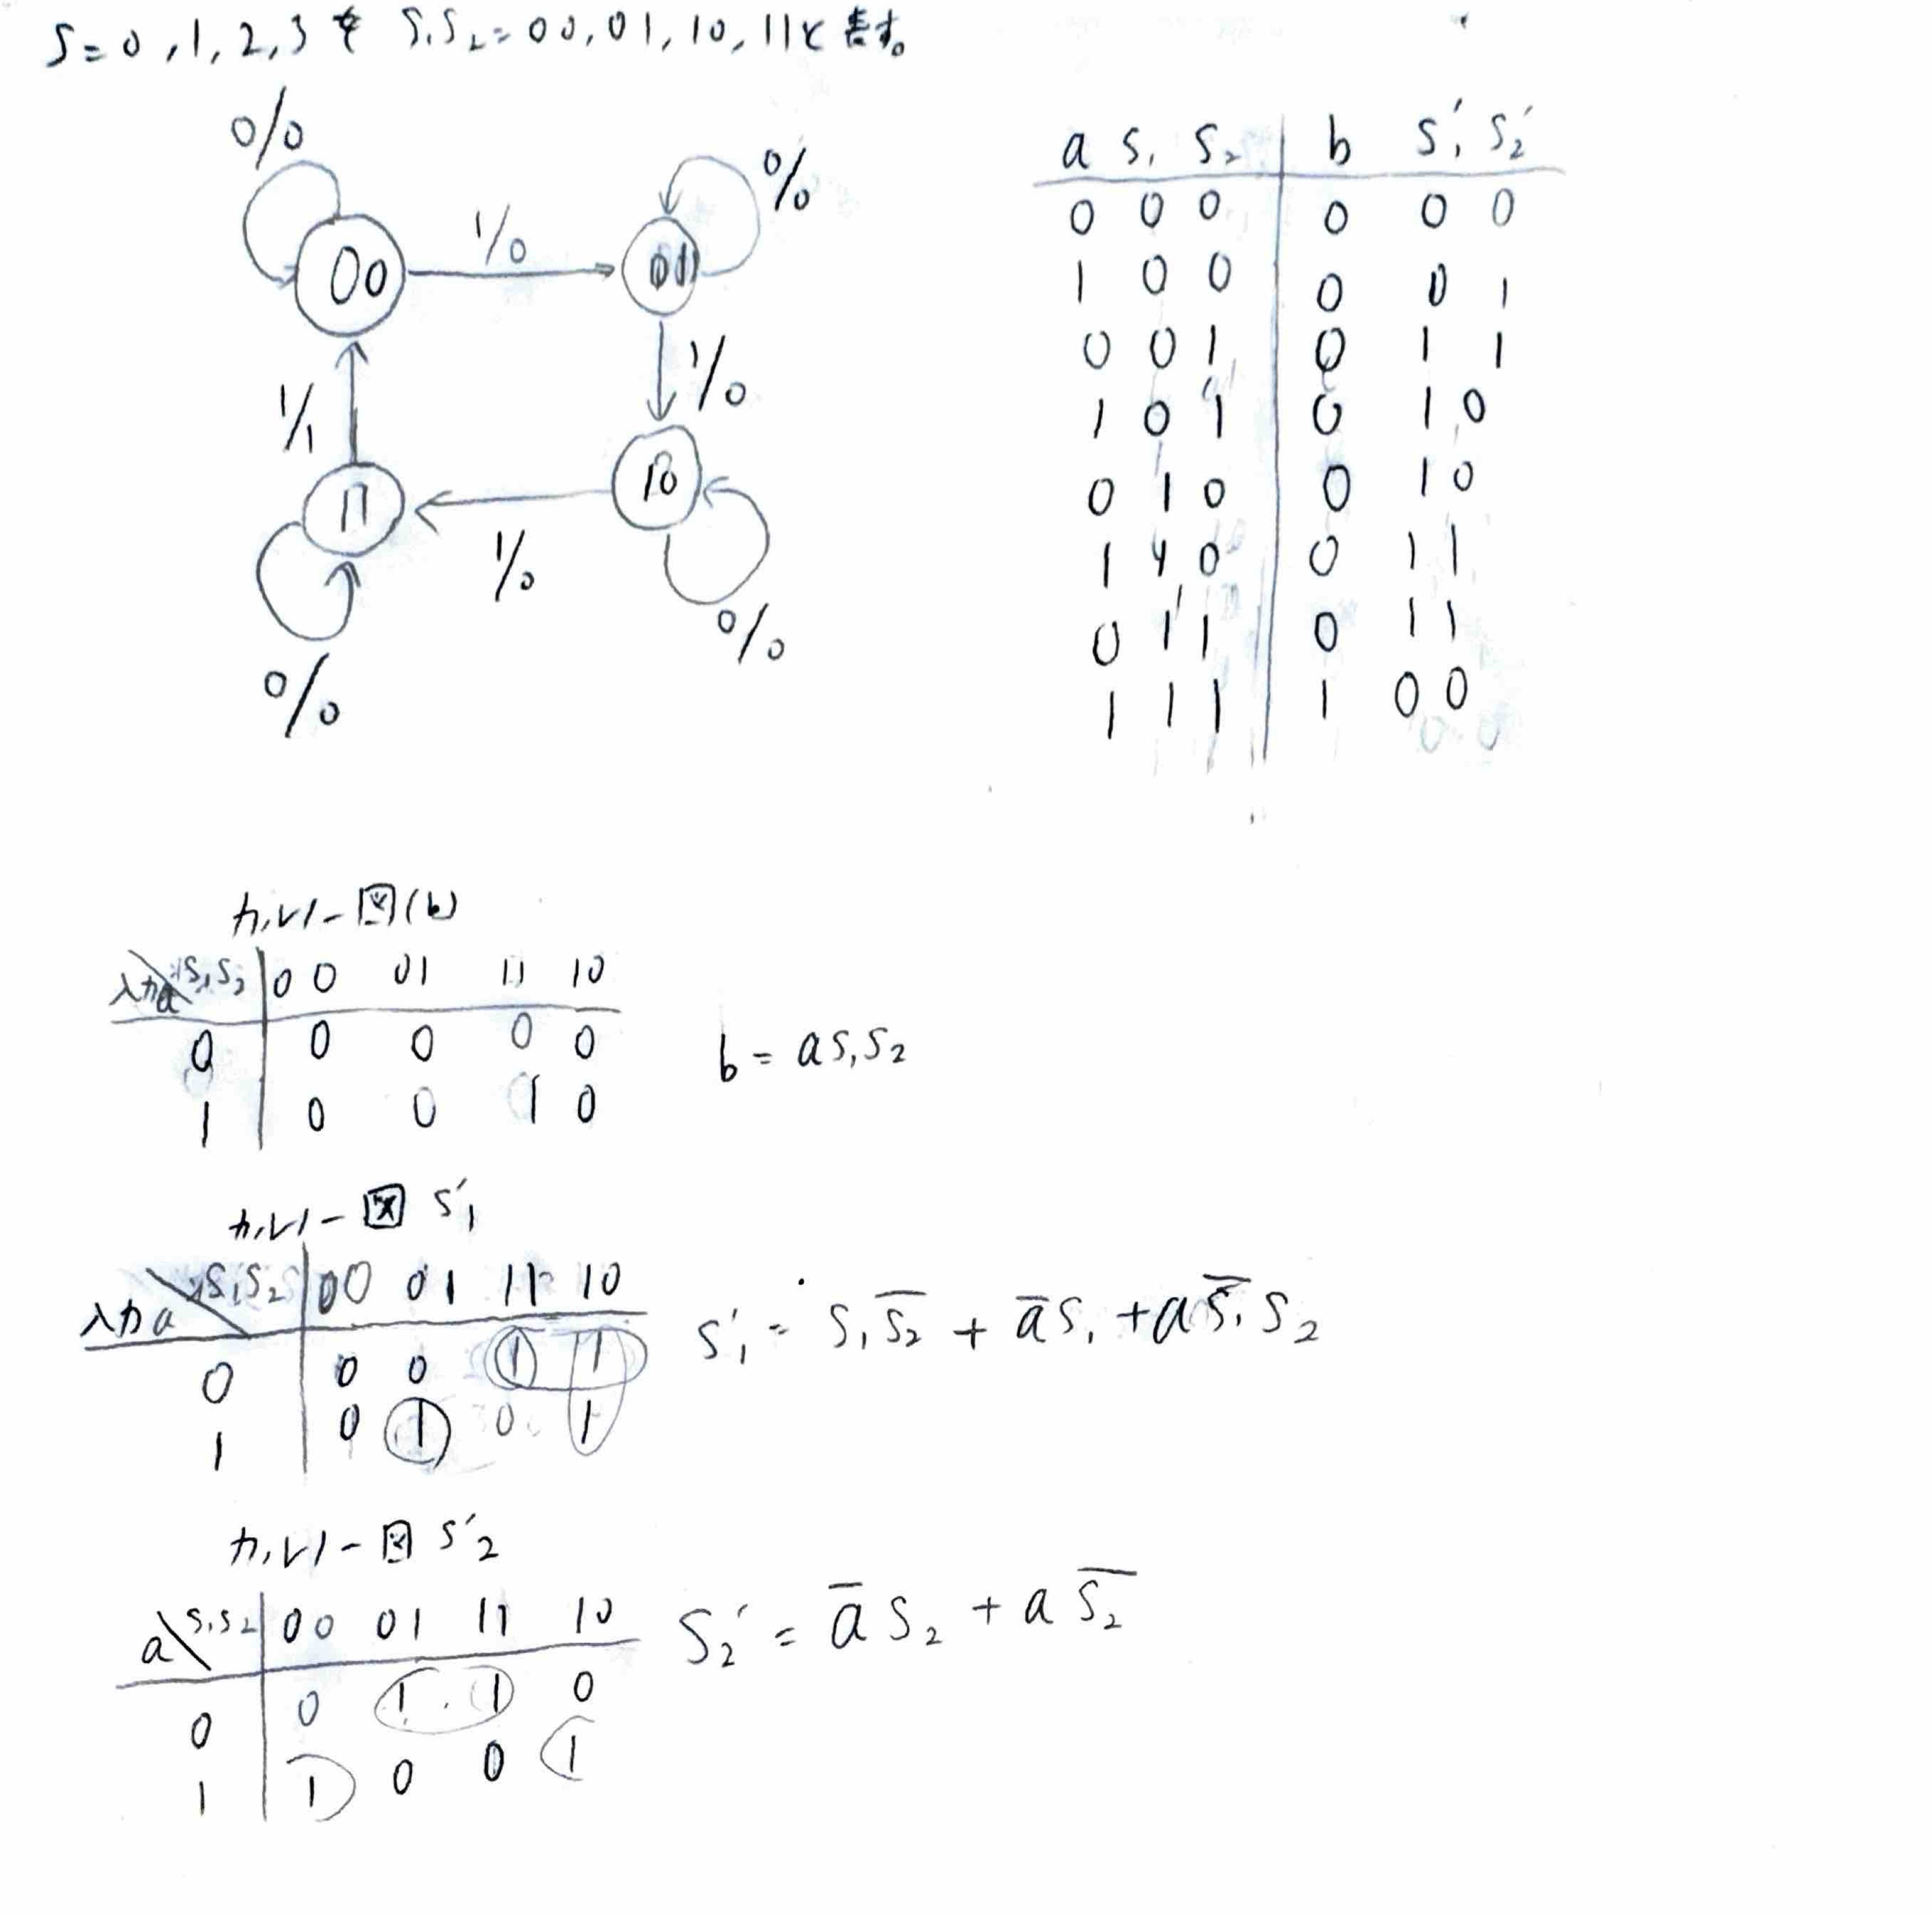
\includegraphics[width=0.8\textwidth]{ex4.jpeg}
	\caption{作成した状態遷移図および真理値表}
	\label{fig:ex4}
\end{figure}

この結果,$b, s1', s2'$の論理式は\ref{eq:ex4}のようになった.

\begin{align}
	\label{eq:ex4}
	\begin{split}
		b   & = a s_1 s_2                                     \\
		s1' & = s_1 \bar{s_2} + \bar{a} s_1 + a \bar{s_1} s_2 \\
		s2' & = \bar{a} s_2 + a \bar{s_2}
	\end{split}
\end{align}


この論理式を下に,\ref{code:mod-count}のようなモジュールcountを作成した.

\begin{lstlisting}[language={Verilog}, caption={モジュールcountのVerilogコード}, label={code:mod-count}]
module count (
    a,ck,b
);
  input a, ck;
  output b;
  wire na;
  wire s1, s2, t;
  wire d1, d2, d3, d4;
  wire e1, e2, e3;
  dffn f1(s1,d1,ck);
  dffn f2(s2,e1,ck);
  assign na = ~a;
  assign ns1 = ~s1;
  assign ns2 = ~s2;

  assign d4 = s1 & ns2, d3 = na & s1, d2 = a & ns1 & s2, d1 = d4 | d3 | d2;
  assign e3 = na & s2, e2 = a & ns2, e1 = e3 | e2;
  assign b = a & s1 & s2;
endmodule
\end{lstlisting}

また,このモジュールcountをシミュレーションするモジュールcountSimを\ref{code:mod-countsim}のように作成した.
clkが発するクロック信号は50サイクル周期で切り替わる.ここで$a$の値を切り替える間隔を100サイクルにすることで,
$a$を1回切り替える間にclkが0,1両方の場合をテストできた.
これにより,少ない行数でより多くのテストケースをカバーできた.

\begin{lstlisting}[language={Verilog}, caption={モジュールcountSimのVerilogコード}, label={code:mod-countsim}]
module countSim;
  reg a;
  wire b;

  clk clk1(ck);
  count dut (a,ck,b);

  initial
    begin
    $dumpfile("countSim.vcd");
    $dumpvars(0, countSim);
    $monitor("%b  %b %b  %b  %b", a, ck, b, dut.s1, dut.s2, $stime);
    $display("a ck b s1 s2       time");

    a = 0;
    #100 a = 1;
    #100 a = 0;
    #100 a = 1;
    #100 a = 0;
    #100 a = 1;
    #100 a = 0;
    #100 a = 1;
    #100 a = 0;
    $finish;
    end
endmodule
\end{lstlisting}

このテストの出力から,状態$s1$と$s2$が正しく遷移していることが確認できた.
また,gtkwaveを用いて波形を表示すると\ref{fig:ex4_wave}のようになった.

\begin{figure}[H]
	\centering
	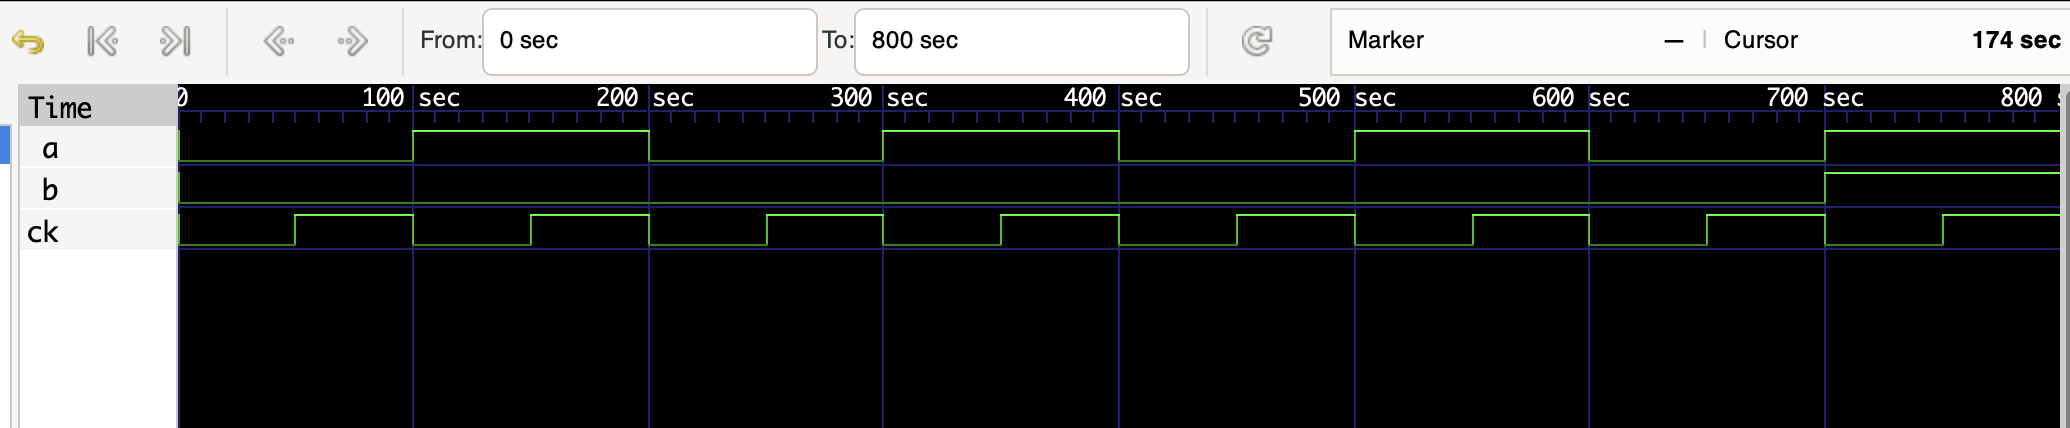
\includegraphics[width=\textwidth]{ex4_wave.png}
	\caption{countSimの波形}
	\label{fig:ex4_wave}
\end{figure}

この波形から,正しい状態遷移の結果$s1s2$が$11$から$00$に遷移するときに$b=1$となっていることが確認できた.

\section{問題5}
\label{sec:ex-5}

実験資料で示された1ビット加算器を参考にして,Nビット加算器モジュールaddNを
\ref{code:mod-addn}のように作成した.

\begin{lstlisting}[language={Verilog}, caption={モジュールaddNのVerilogコード}, label={code:mod-addn}]
module addN (
    a, b, sum, ci, cu
);
  parameter N = 8;

  input [N-1:0] a, b;
  input ci;
  output [N-1:0] sum;
  output cu;

  wire [N-1:0] sum;
  wire [N:0] c; // carries
  assign c[0] = ci;


  assign sum = a ^ b ^ c[N-1:0];
  assign c[N:1] = (a & b) | (b & c[N-1:0]) | (a & c[N-1:0]);


  assign cu = c[N];
endmodule
\end{lstlisting}

また,モジュールaddNをシミュレーションするモジュールaddNSimを\ref{code:mod-addnsim}のように作成した.

\begin{lstlisting}[language={Verilog}, caption={モジュールaddNSimのVerilogコード}, label={code:mod-addnsim}]
module addNSim;
  reg [7:0] a, b;
  reg ci;
  wire [7:0] sum;
  wire cu;
  addN #8 g1(a, b, sum, ci, cu);

  initial begin
    $dumpfile("addN.vcd");
    $dumpvars(0, addNSim);
    $monitor(" %b  %b    %b  %b   %b", a, b,ci, sum, cu, $stime);
    $display("        a         b   ci       sum  cu      time");

    // test normal
    a = 8'b00000011;
    b = 8'b00000011;
    ci = 0;

    // test carry in
    #10;
    a = 8'b00000011;
    b = 8'b00000011;
    ci = 1;

    #10;
    // test overflow
    a = 8'b11111111;
    b = 8'b00000001;
    ci = 0;

    #10 $finish;
  end
endmodule
\end{lstlisting}

このテストの出力は下のようになった.

\begin{verbatim}
a                b   ci       sum  cu      time
00000011  00000011    0  00000110   0         0
00000011  00000011    1  00000111   0        10
11111111  00000001    0  00000000   1        20
\end{verbatim}

また,gtkwaveを用いて波形を表示すると\ref{fig:ex5}のようになった.

\begin{figure}[H]
	\centering
	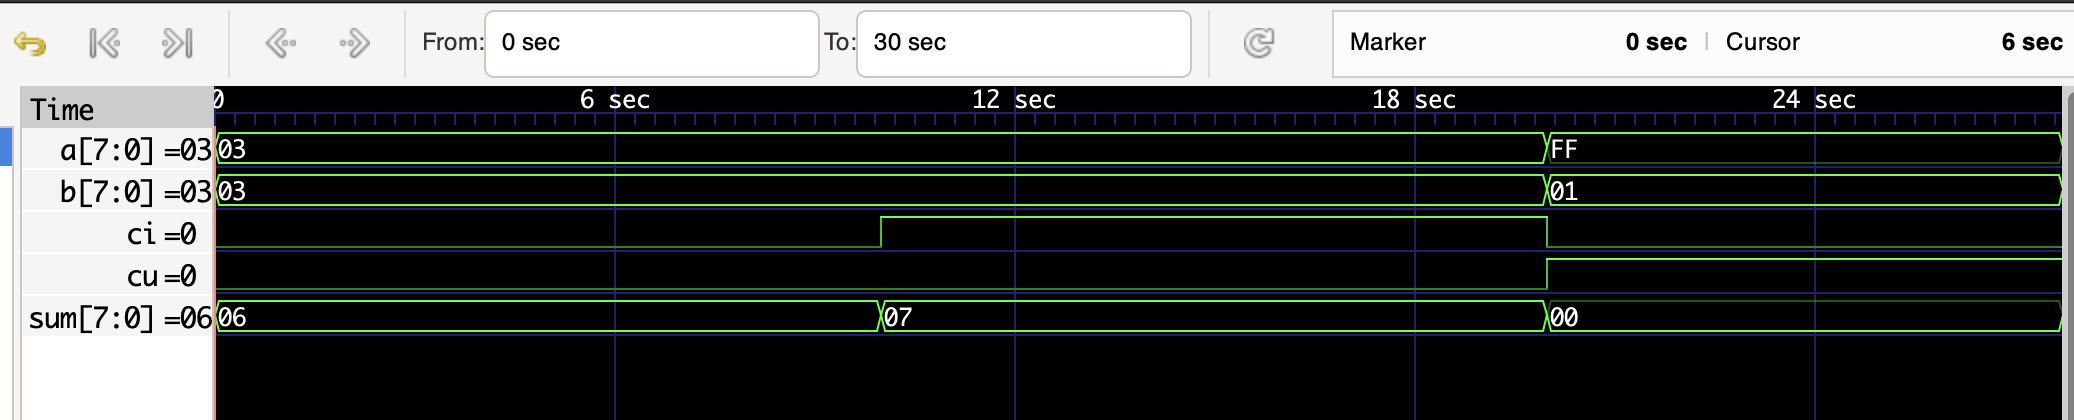
\includegraphics[width=\textwidth]{ex5.png}
	\caption{addNSimの波形}
	\label{fig:ex5}
\end{figure}

これらの結果から,通常の演算と桁あふれが発生する演算の両方でモジュールaddNが正しく動作していることが確認できた.
ビットベクトルを用いることで,1ビット加算器の実装を大きく変えることなくNビット加算器を実装できることがわかった.

\section{問題6}
\label{sec:ex-6}

実験資料で示された1ビットレジスタを参考にして,NビットレジスタregNを作成した.

\subsection{モジュールdffnの改良}

まず,モジュールdffnをNビットの入出力に対応させる必要があると考え,\ref{code:mod-dffn}のように改良した.
なお,入出力ビット数Nのデフォルト値を1にすることで既にモジュールdffnを使用している他のモジュールに影響を与えないようにした.

\begin{lstlisting}[language={Verilog}, caption={改良後のモジュールdffnのVerilogコード}, label={code:mod-dffn}]
module dffn (
    Q,D,ck
);
  parameter N = 1;

  input [N-1:0] D;
  input ck;
  output [N-1:0] Q;
  reg [N-1:0] Q;
  initial
      Q = {N{1'b0}};
  always @(negedge ck)
      Q = D;
endmodule
\end{lstlisting}

あわせて,モジュールdffnをシミュレーションするモジュールdffnSimも\ref{code:mod-dffnsim}のように改良した.

\begin{lstlisting}[language={Verilog}, caption={改良後のモジュールdffnSimのVerilogコード}, label={code:mod-dffnsim}]
module dffnSim;
  reg[1:0] i;
  wire[1:0] o;
  clk clk1(ck);
  dffn #2 dffn1(o, i, ck);
  initial
    begin
    $dumpfile("dffnSim.vcd");
    $dumpvars(0, dffnSim);
    $monitor(" %b %b %b", ck,i,o,$stime);
    $display("ck  i  o      time");
    i = 2'b00;
    #100 i = 2'b01;
    #200 i = 2'b10;
    #100 $finish;
    end
endmodule
\end{lstlisting}

このテストの出力は下のようになった.

\begin{verbatim}
 ck  i  o      time
 0 00 00         0
 1 00 00        50
 0 01 01       100
 1 01 01       150
 0 01 01       200
 1 01 01       250
 0 10 10       300
 1 10 10       350
dffnSim.v:15: $finish called at 400 (1s)
 0 10 10       400
\end{verbatim}

gtkwaveを用いて波形を表示すると\ref{fig:ex6}のようになった.

\begin{figure}[H]
	\centering
	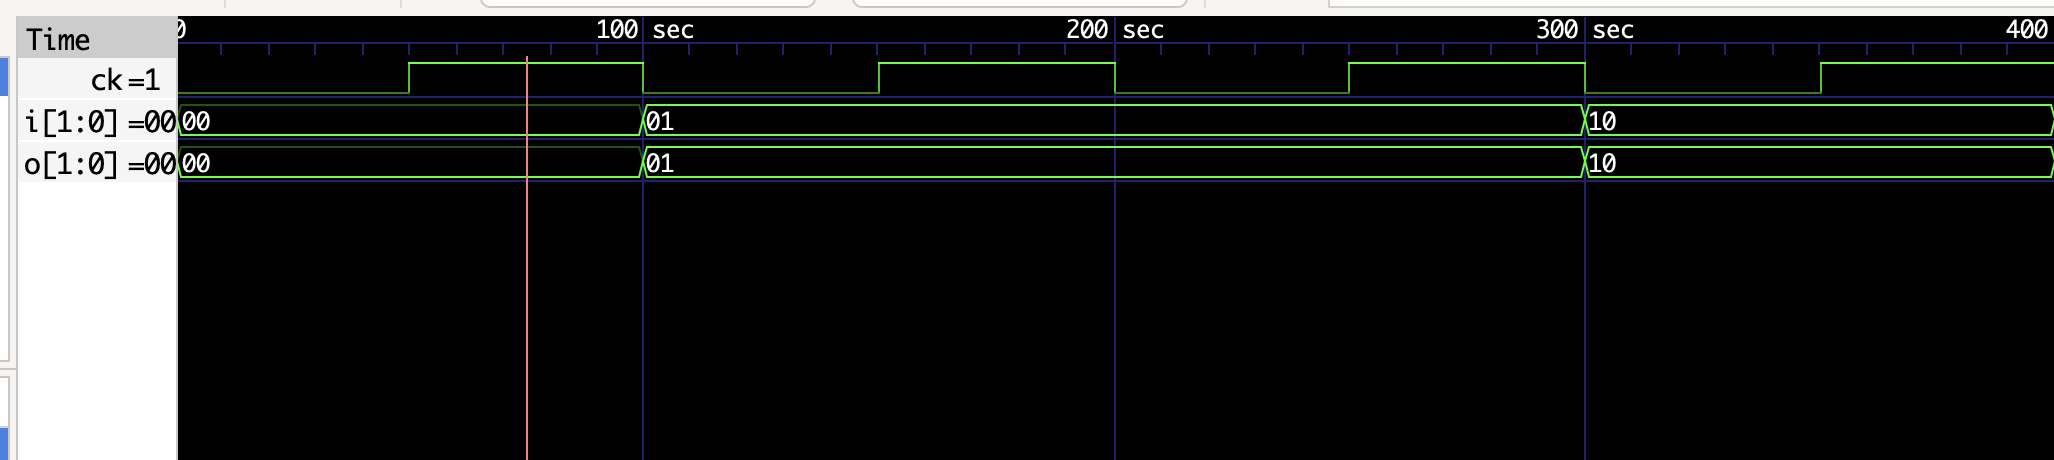
\includegraphics[width=\textwidth]{ex6-dffn.png}
	\caption{dffnSimの波形}
	\label{fig:ex6}
\end{figure}

このテストでは2ビットの信号の入出力をテストしている.
クロックの立ち下がりに同期して2ビットの値を更新・保持できているので,仕様を崩すことなくモジュールdffnをNビット入出力に対応させることができたと判断した.

\subsection{モジュールregNの作成}

次に,NビットレジスタのモジュールregNを\ref{code:mod-regn}のように作成した.

\begin{lstlisting}[language={Verilog}, caption={モジュールregNのVerilogコード}, label={code:mod-regn}]
module regN (
    l, d, ck, q
);
  parameter N = 8;

  input l;
  input [N-1:0] d;
  input ck;
  output [N-1:0] q;
  wire [N-1:0] d1;

  dffn #8 f1(q,d1,ck);
  assign d1 = l ? d : q;
endmodule
\end{lstlisting}

実験資料で示されたconditional assignを用いることで,少ない記述量でも
load信号の値に応じて$d1$に送られる信号を制御することができた.

また,モジュールregNをシミュレーションするモジュールregNSimを\ref{code:mod-regnsim}のように作成した.

\begin{lstlisting}[language={Verilog}, caption={モジュールregNSimのVerilogコード}, label={code:mod-regnsim}]
  module regNSim ();
  reg l;
  reg [7:0] d;
  clk c1(ck);
  wire [7:0] q;

  regN #8 g1(l, d, ck, q);

  initial begin
  $dumpfile("regN.vcd");
  $dumpvars(0, regNSim);
  $monitor("   %b    %b  %b %b", l, d, ck, q, $stime);
  $display("load        data ck        q      time");

  l = 0;
  d = 8'b00000000;
  #50;

  // pass first data
  l = 1;
  d = 8'b00000011;
  #50;

  // get first data
  l = 0;
  #50;

  // pass second data
  l = 1;
  d = 8'b00001111;
  #50;

  // get second data
  l = 0;
  #50;

  #50 $finish;
  end
endmodule
\end{lstlisting}

このテストの出力は下のようになった.

\begin{verbatim}
load        data ck        q      time
   0    00000000  0 00000000         0
   1    00000011  1 00000000        50
   0    00000011  0 00000011       100
   1    00001111  1 00000011       150
   0    00001111  0 00001111       200
   0    00001111  1 00001111       250
   0    00001111  0 00001111       300
regNSim.v:39: $finish called at 300 (1s)
\end{verbatim}

gtkwaveを用いて波形を表示すると\ref{fig:ex6-wave}のようになった.

\begin{figure}[H]
	\centering
	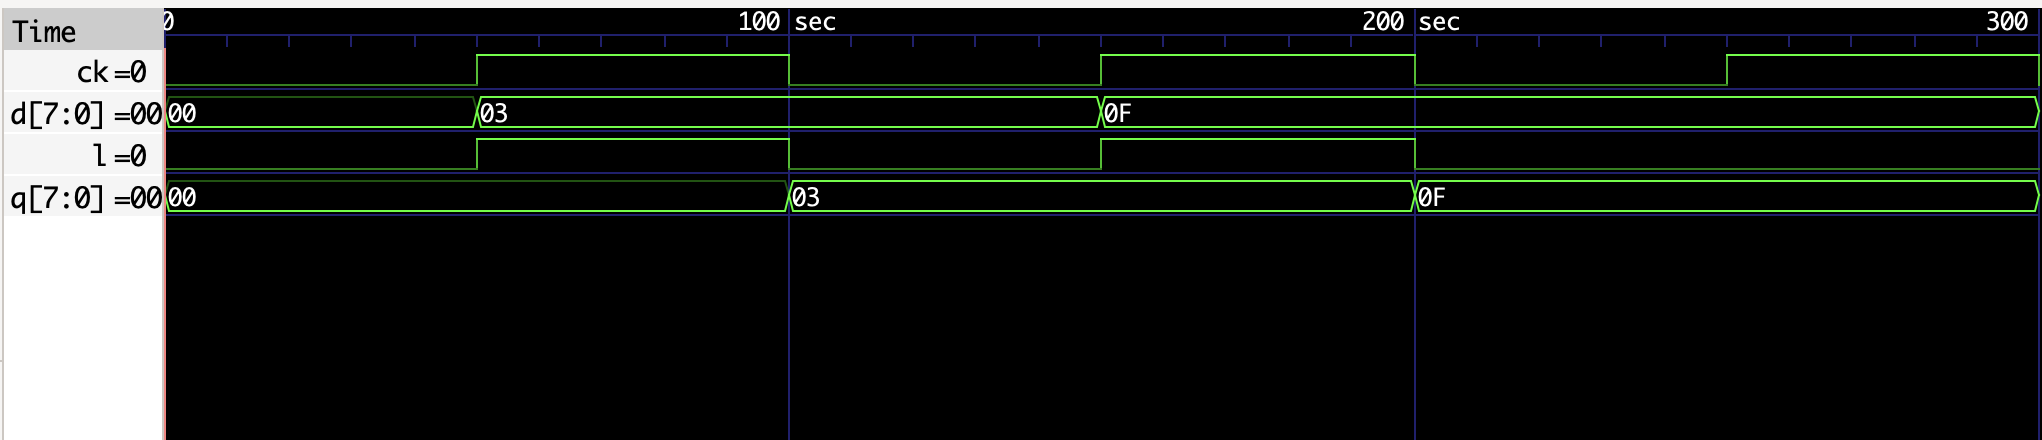
\includegraphics[width=\textwidth]{ex6-wave.png}
	\caption{regNSimの波形}
	\label{fig:ex6-wave}
\end{figure}

クロックが立ち下がる際にloadに1が入力されているときだけ,出力$q$が$d$の値に更新されることが視覚的に確認できた.

\section{問題7}

実験資料で示されたNビット加減算器の図解を参考にして,Nビット加減算器calcNを\ref{code:mod-calcn}のように作成した.

\begin{lstlisting}[language={Verilog}, caption={モジュールcalcNのVerilogコード}, label={code:mod-calcn}]
module calcN (
  a, b, sum, k, cu
);
  parameter N = 8;

  input [N-1:0] a, b;
  input k;
  output [N-1:0] sum;
  output cu;

  wire[N-1:0] B = k ? ~b : b;
  addN #(
      .N(N)
  ) g1(a, B, sum, k, cu);

endmodule
\end{lstlisting}

また,モジュールcalcNをシミュレーションするモジュールcalcNSimを\ref{code:mod-calcsim}のように作成した.

\begin{lstlisting}[language={Verilog}, caption={モジュールcalcNSimのVerilogコード}, label={code:mod-calcsim}]
  module calcNSim;
  reg [7:0] a, b;
  reg k;
  wire [7:0] sum;
  wire cu;
  calcN #8 g1(a, b, sum, k, cu);

  initial begin
    $dumpfile("calcN.vcd");
    $dumpvars(0, calcNSim);
    $monitor(" %b  %b  %b  %b  %b", a, b, k, sum, cu, $stime);
    $display("        a         b  k       sum  cu      time");

    // test add
    a = 8'b00000011;
    b = 8'b00000011;
    k = 0;

    // test sub
    #10;
    a = 8'b00000011;
    b = 8'b00000011;
    k = 1;
    #10;

    // test add overflow
    a = 8'b11111111;
    b = 8'b00000001;
    k = 0;
    #10;

    // test sub overflow
    a = 8'b00000000;
    b = 8'b00000001;
    k = 1;
    #10 $finish;
  end
endmodule
\end{lstlisting}

このテストの出力は下のようになった.

\begin{verbatim}
        a         b  k       sum  cu      time
 00000011  00000011  0  00000110  0         0
 00000011  00000011  1  00000001  1        10
 11111111  00000001  0  00000000  1        20
 00000000  00000001  1  11111111  0        30
calcNSim.v:41: $finish called at 40 (1s)
\end{verbatim}

$k = 0$のときに加算,$k = 1$のときに減算を行うことが確認できた.
また,加算時は$cu=1$ならオーバーフロー,減算時は$cu=0$ならアンダーフローとなることも確認できた.

gtkwaveを用いて波形を表示すると\ref{fig:ex7}のようになった.
$a$と$b$に同じ入力をしていても,$k$を切り替えることで加算減算が切り替わり異なる値を正しく出力していることが確認できた.

\begin{figure}[H]
	\centering
	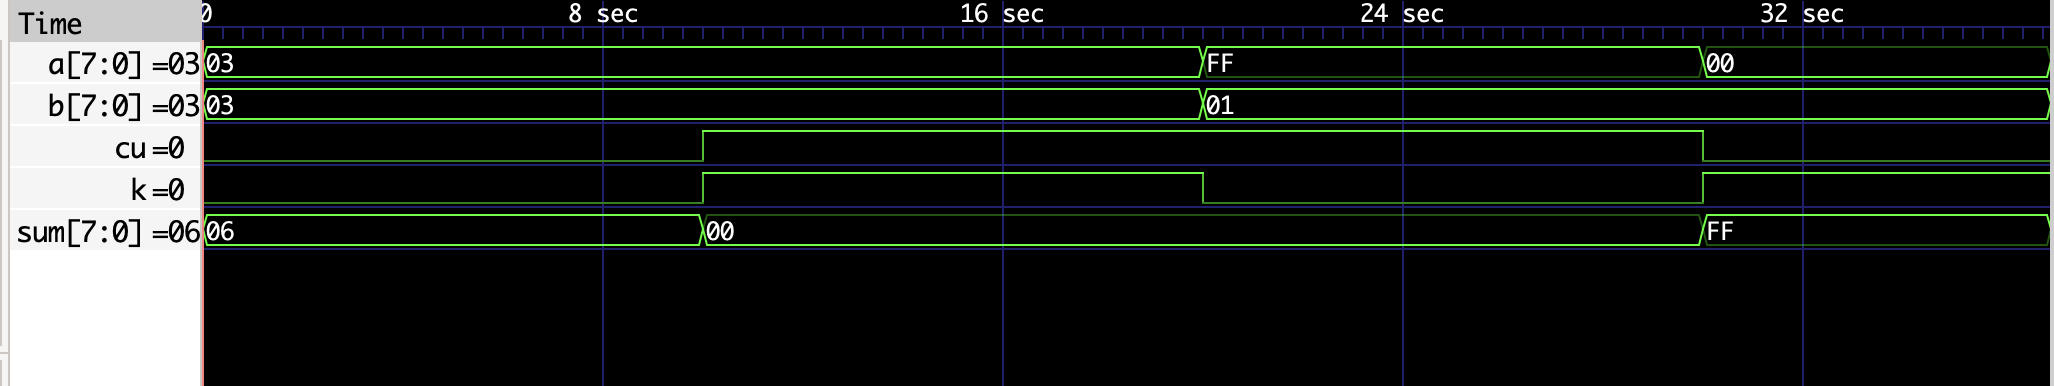
\includegraphics[width=\textwidth]{ex7-wave.png}
	\caption{calcNSimの波形}
	\label{fig:ex7}
\end{figure}

% \bibliography{hoge} %hoge.bibから拡張子を外した名前
% \bibliographystyle{junsrt} %参考文献出力スタイル
% 使用する際は latex-workshop.latex.recipe.default を
% ptex2pdf (uplatex) → bibtex → ptex2pdf (uplatex) × 2
% に変更

\end{document}
